\documentclass[12pt,a4paper]{article}
\usepackage[english]{babel}
\usepackage[utf8]{inputenc}
\usepackage{fancyhdr}
\usepackage{hyperref}


% Math
\usepackage{bm}

% graphics
\usepackage{graphicx}
\graphicspath{ {images/} }
\usepackage{tikz}

% date
\usepackage{datetime}
\newdateformat{specialdate}{\THEYEAR-\twodigit{\THEMONTH}-\twodigit{\THEDAY}}
\date{\specialdate\today}
\usepackage{xcolor}

% Colors
\definecolor{command}{rgb}{0.325, 1, 1}
\definecolor{flag}{rgb}{1, 0.325, 0.325}
\definecolor{param}{rgb}{0.825, 0.825, 0.825}

\definecolor{info}{rgb}{0.825, 0.825, 0.825}
\definecolor{ok}{rgb}{0.125, 0.825, 0.125}
\definecolor{redirection}{rgb}{0.825, 0.825, 0.125}
\definecolor{bad}{rgb}{0.825, 0.125, 0.125}

%renew commands
\renewcommand{\contentsname}{Tabla de contenidos}

\begin{document}
	\begin{titlepage}
		\centering
		
\includegraphics[width=0.4\textwidth]{logo-ugr.png}\\*
		{\scshape\LARGE Universidad de Granada \par}
		{\large \date{\specialdate\today}\par}
		\vspace{1cm}
		{\LARGE\bfseries Práctica 4\par}
		\vspace{1.5cm}
		{\scshape\large Ingeniería de Servidores\par}
		\vspace{2cm}
		{\Large\itshape Lukas Häring García 3ºC\par}
	\end{titlepage}
	
	\tableofcontents
	
	\newpage
	
	
	%\begin{figure}[h]
	%	\centering
	%	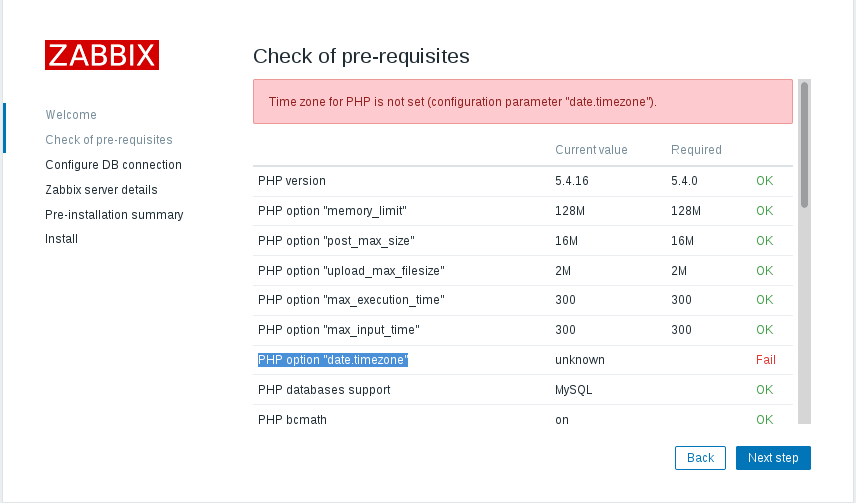
\includegraphics[width=1.0\textwidth]{images/timezone.png}
	%	\caption{Error date.timezone}
	%\end{figure}
	
	%\begin{tikzpicture}[node distance=-0.5em]
	%\node[anchor=north,draw=black,fill=black,inner xsep=0.5cm,inner ysep=0.2cm,line width=4pt,text width=\textwidth - 1cm,align=left] (box) { {\color{command}\textbf{cat}} {\color{param} /var/log/audit/audit.log} {\color{flag} $\mid$} {\color{command}\textbf{grep}} {\color{param} zabbix\_agentd} {\color{flag} $\mid$} {\color{command}\textbf{grep}} {\color{param} denied} {\color{flag} $\mid$} {\color{command}\textbf{audit2allow}} {\color{flag} -M} {\color{param} zabbix\_agent\_setrlimit}};
	%\node[fill=black,rounded corners] at (box.west) {\color{white}$\boldsymbol{>}$};
	%\end{tikzpicture}
	
	\section{Phoronix}
	Phoronix Test Suite es la plataforma de pruebas y evaluación comparativa más completa disponible para Linux
	\newline
	\newline
	El primer test, es para la CPU, consiste en resolver un número de sudokus y devuelve la media de los tiempos.
	\newline
	\newline
	El tiempo medio obtenido es de 25 segundos aproximadamente en nuestra máquina virtual de Ubuntu.
	\begin{figure}[h]
		\centering
		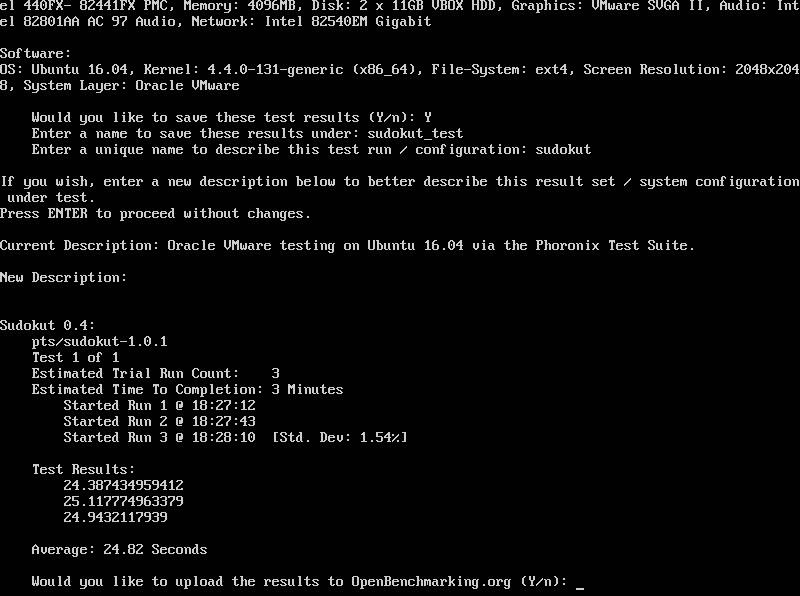
\includegraphics[width=1.0\textwidth]{images/sudokut-ubuntu-test.png}
		\caption{Test CPU, Resolución de sudoku}
	\end{figure}
	\newpage
	El segundo test se trata de introducir una gran cantidad de enteros en la RAM y sacarlos, así comprobar la velocidad de nuestra memoria (ancho de banda).
	\newline
	\newline
	El test es realizado una única vez, con un tiempo estimado de 11 minutos.
	\newline
	\newline
	El resultado obtenido fue de 9052.47 MB/s de ancho de banda.
	\begin{figure}[h]
		\centering
		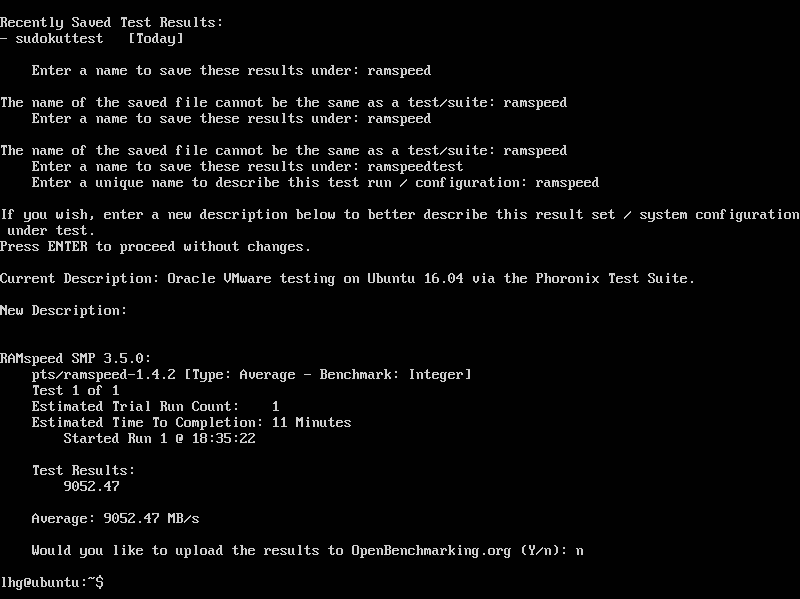
\includegraphics[width=1.0\textwidth]{images/ramspeed-ubuntu-test.png}
		\caption{Test memoria RAM, Entrada y salida de valores enteros}
	\end{figure}

	\newpage
	\section{JMeter}
	Apache JMeter es un software de código abierto, diseñada para cargar el comportamiento funcional de las pruebas y medir el rendimiento.
	
	\subsection{Instalación en Ubuntu Server}
	
	Suponiendo que tenemos la \textbf{primera práctica} acabada.
	\newline
	\newline
	Descargamos \textbf{docker-compose} en nuestra máquina,
	\newline
	\newline
	
\begin{tikzpicture}[node distance=-0.5em]
	\node[anchor=north,draw=black,fill=black,inner xsep=0.5cm,inner ysep=0.2cm,line width=4pt,text width=\textwidth - 1cm,align=left] (box) { {\color{command}\textbf{apt}} {\color{flag} install} {\color{param} docker-compose}};
	\node[fill=black,rounded corners] at (box.west) {\color{white}$\boldsymbol{>}$};
	\end{tikzpicture}
	\newline
	\newline
	Una vez instalado, nos vamos a realizar un \textbf{git pull} del proyecto de \textit{David Palomar}.
	\newline
	\newline
	
\begin{tikzpicture}[node distance=-0.5em]
	\node[anchor=north,draw=black,fill=black,inner xsep=0.5cm,inner ysep=0.2cm,line width=4pt,text width=\textwidth - 1cm,align=left] (box) { {\color{command}\textbf{git}} {\color{flag} clone} {\color{param} https://github.com/davidPalomar-ugr/iseP4JMeter.git}};
	\node[fill=black,rounded corners] at (box.west) {\color{white}$\boldsymbol{>}$};
	\end{tikzpicture}
	\newline
	\newline
	Ahora tendremos una carpeta llamada "\textit{iseP4JMeter}", tras entrar en ella, podemos ejecutar el \textit{Docker}.
	\newline
	\newline
	\textbf{Nota:} En diferentes pruebas he tenido que realizar un reinicio previo de la máquina antes de abrir el \textit{Docker}.
	\newline
	\newline
	
\begin{tikzpicture}[node distance=-1.5em]
	\node[anchor=north,draw=black,fill=black,inner xsep=2.0cm,inner ysep=0.2cm,line width=4pt,text width=\textwidth - 5.5cm,align=left] (box) { {\color{command}\textbf{docker-compose}} {\color{flag} up - d}};
	\node[fill=black,rounded corners] at (box.west) {\color{white}$\boldsymbol{iseP4JMeter >}$};
	\end{tikzpicture}
	\newline
	\newline
	Podemos realizar una prueba previa, que realizará una petición "HTTP" para comprobar que nos devuelve un resultado.
	\newline
	\newline
	
\begin{tikzpicture}[node distance=-1.5em]
	\node[anchor=north,draw=black,fill=black,inner xsep=2.0cm,inner ysep=0.2cm,line width=4pt,text width=\textwidth - 5.5cm,align=left] (box) { {\color{command}\textbf{sh}} {\color{param} pruebaEntorno.sh}};
	\node[fill=black,rounded corners] at (box.west) {\color{white}$\boldsymbol{iseP4JMeter >}$};
	\end{tikzpicture}
	\newpage
	
	\subsection{Setup de JMeter}
	Se ha realizado la práctica en el sistema operativo \textbf{Windows}, pero en realidad no existe ninguna diferencia.
	\newline
	\newline
	Comentar previamente que se utiliza el click derecho para "\textbf{Añadir}" un nuevo elemento en nuestro entorno.
	\begin{figure}[h]
		\centering
		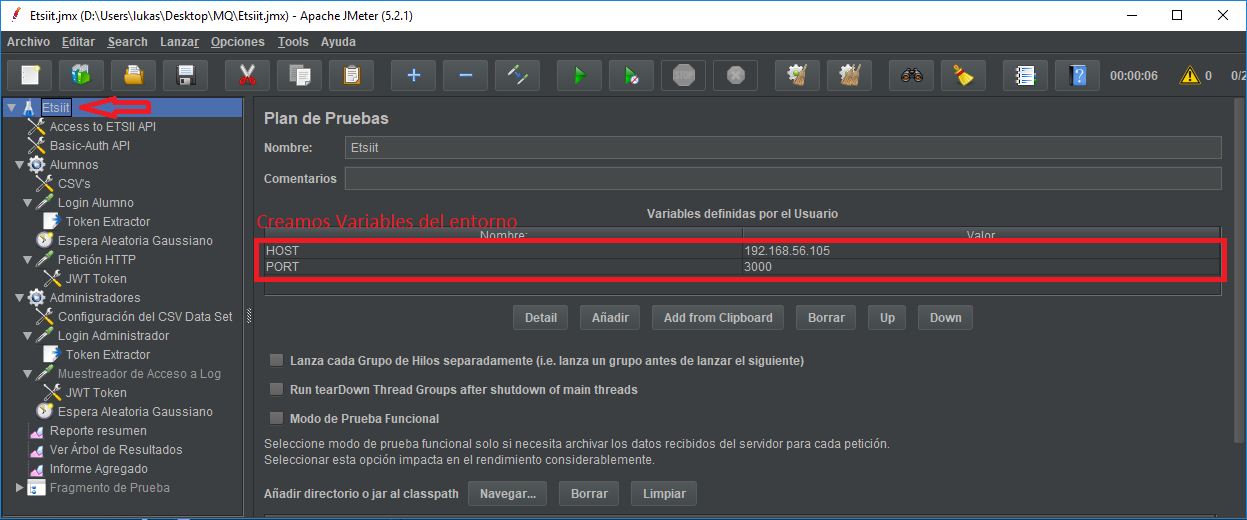
\includegraphics[width=1.0\textwidth]{images/step-1.png}
		\caption{Primer paso, creación de variables del entorno}
	\end{figure}
	Añadimos previamente la configuración HTTP de nuestro archivo.
	\begin{figure}[h]
		\centering
		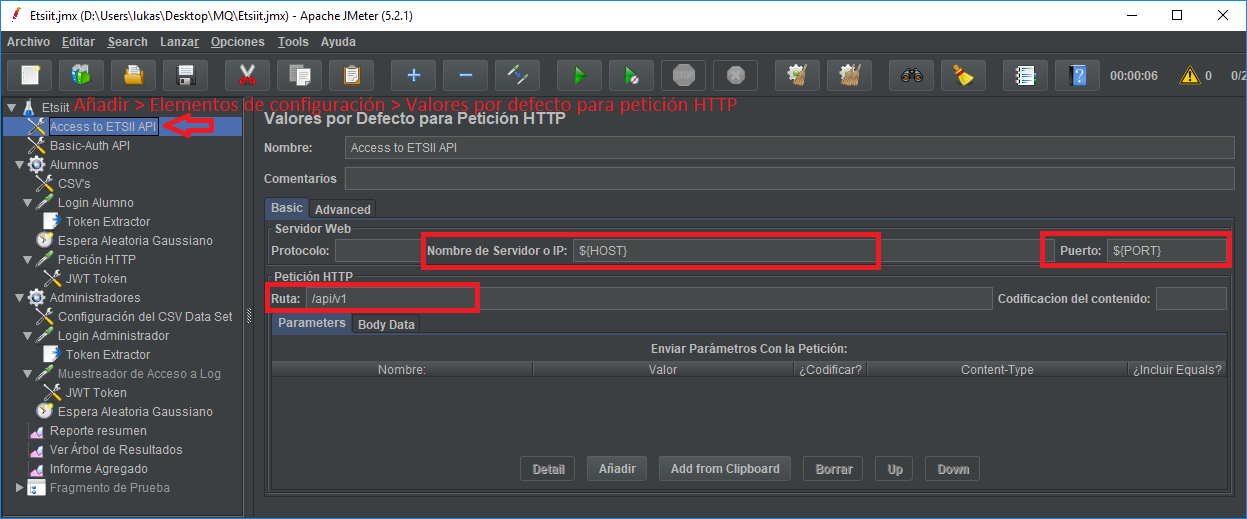
\includegraphics[width=1.0\textwidth]{images/step-2.png}
		\caption{Segundo paso, valores por defecto}
	\end{figure}

	\newpage

	\begin{figure}[h]
		\centering
		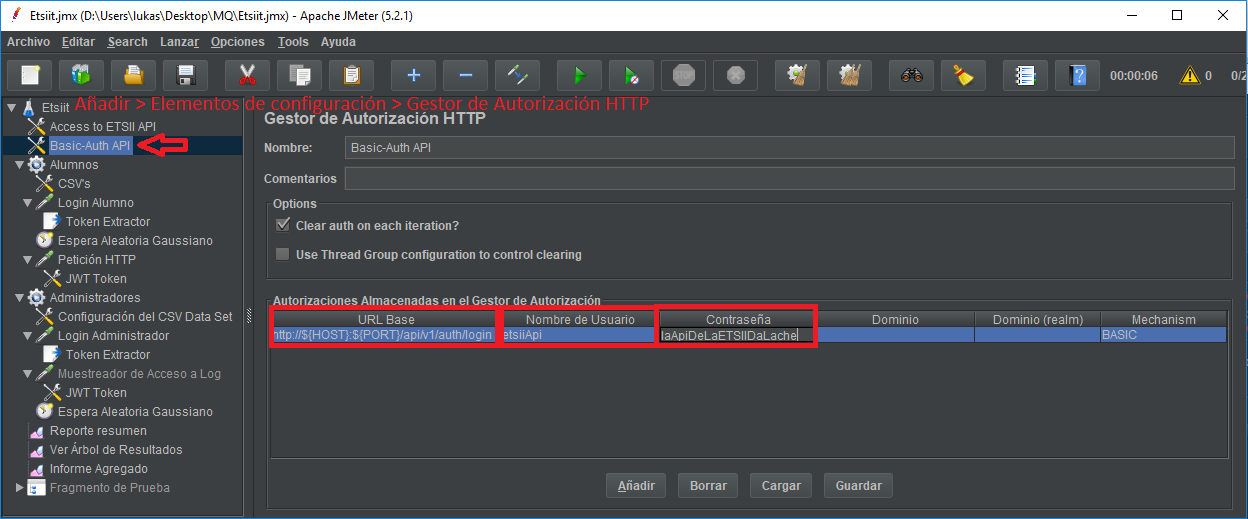
\includegraphics[width=1.0\textwidth]{images/step-3.png}
		\caption{Tercer paso, Autorización HTTP}
	\end{figure}
	Creamos \textbf{dos grupos de hebras} "Alumnos" y "Administradores", cuyos valores son modificables.

	\begin{figure}[h]
		\centering
		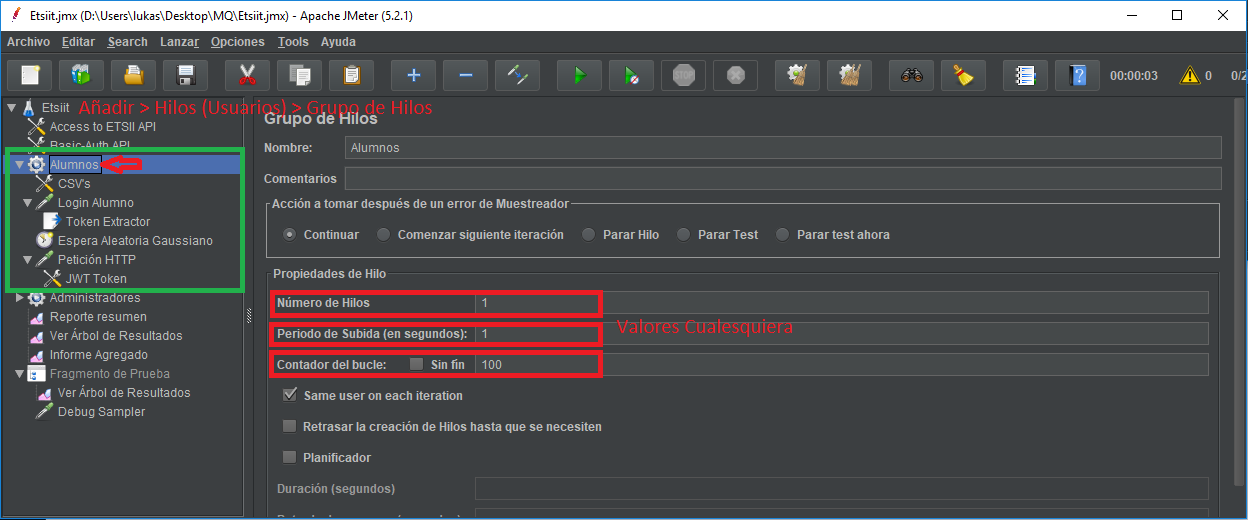
\includegraphics[width=1.0\textwidth]{images/step-4.png}
		\caption{Primer paso, creación de variables del entorno}
	\end{figure}
	
	\newpage
	Asignamos para cada grupo de hebras, su CSV correspondiente.
	\begin{figure}[h]
		\centering
		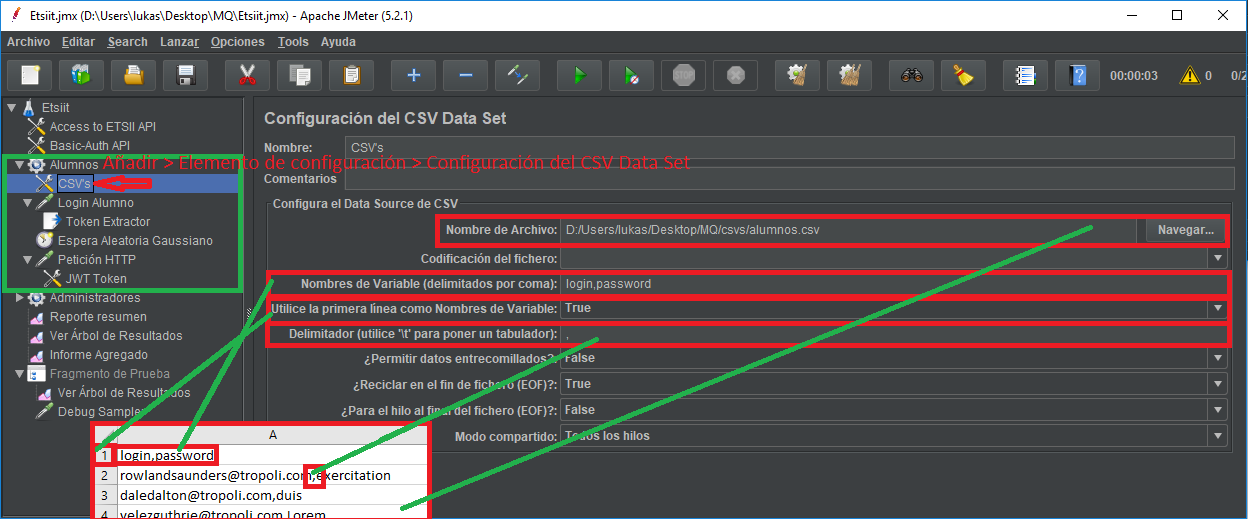
\includegraphics[width=1.0\textwidth]{images/step-5.png}
		\caption{Quinto paso, asignar archivos CSV}
	\end{figure}

	Cada entrada del CSV va a realizar una petición HTTP, por lo que vamos a utilizar dichos valores para generarla.

	\begin{figure}[h]
		\centering
		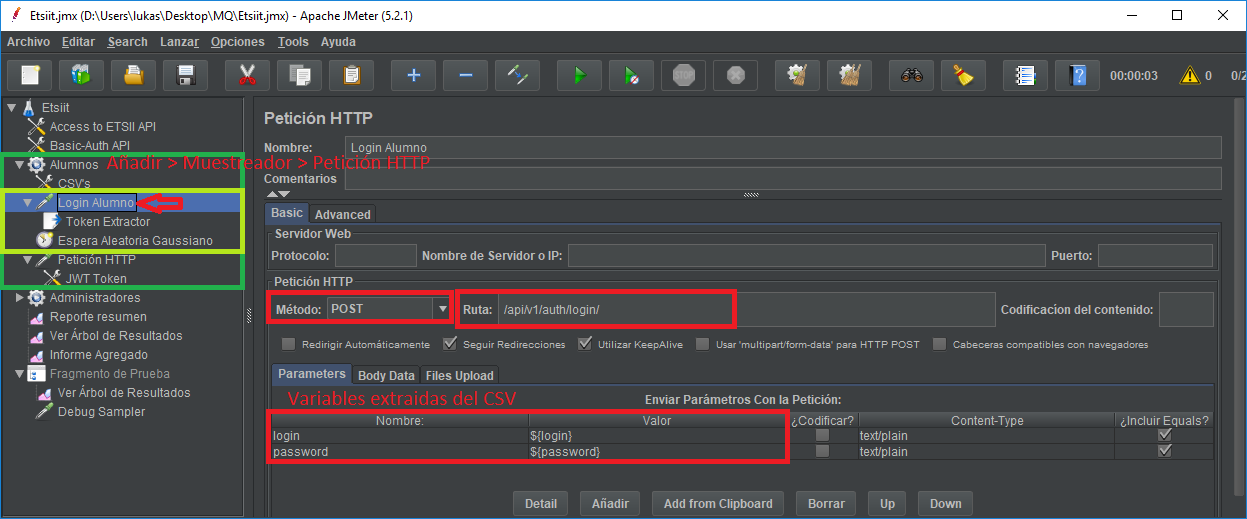
\includegraphics[width=1.0\textwidth]{images/step-6.png}
		\caption{Sexto, Peticiones HTTP de cada muestra}
	\end{figure}

	\newpage
	
	Cada petición a su vez, nos va a devolver un "\textbf{token}" correspondiente.
	
	\begin{figure}[h]
		\centering
		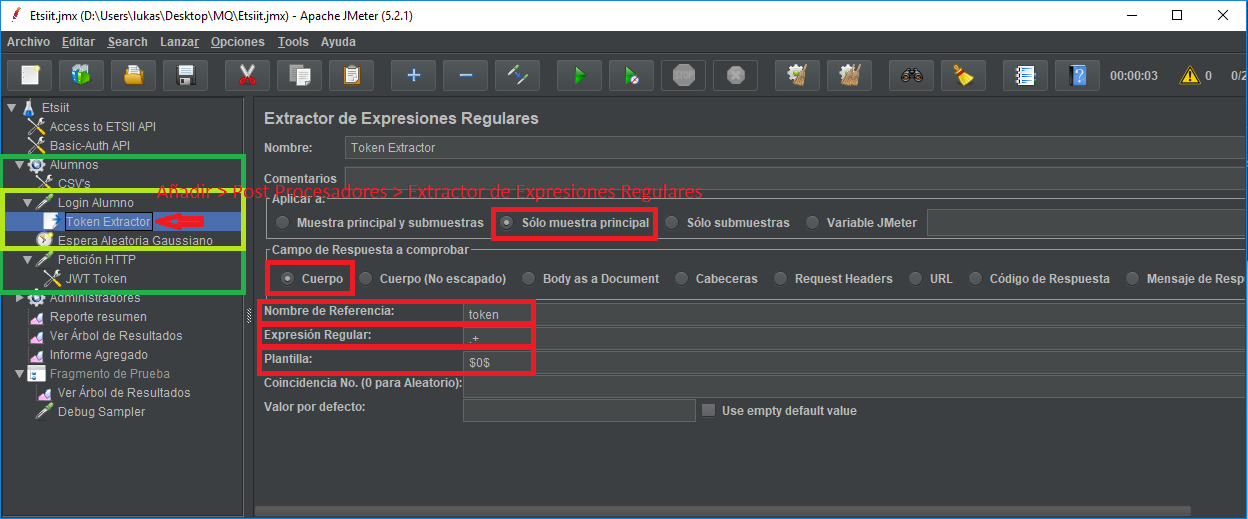
\includegraphics[width=1.0\textwidth]{images/step-7.png}
		\caption{Séptimo, Extracción del token}
	\end{figure}

	Se realizará una \textbf{espera aleatoria} después de dicha extracción.

	Vamos a utilizar el token extraído para extraer finalmente el \textbf{token de Acceso} a dicho usuario.

	\begin{figure}[h]
		\centering
		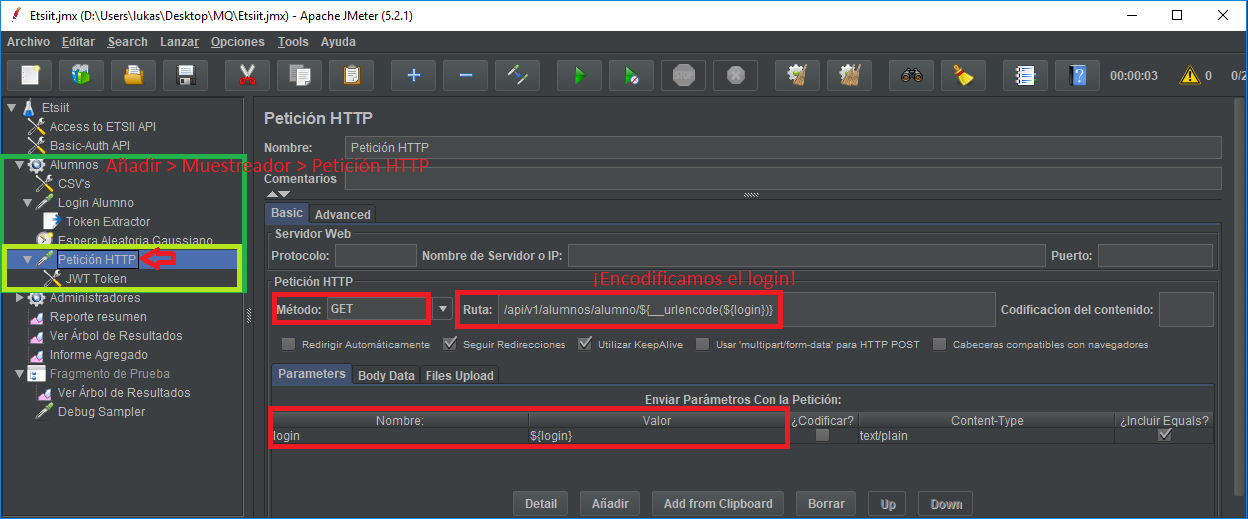
\includegraphics[width=1.0\textwidth]{images/step-8.png}
		\caption{Octavo paso, petición del token JWT}
	\end{figure}

	\newpage

	Añadimos a la cabecera la \textbf{autentificación} de tipo \textbf{Bearer} con el \textbf{token} obtenido.

	\begin{figure}[h]
		\centering
		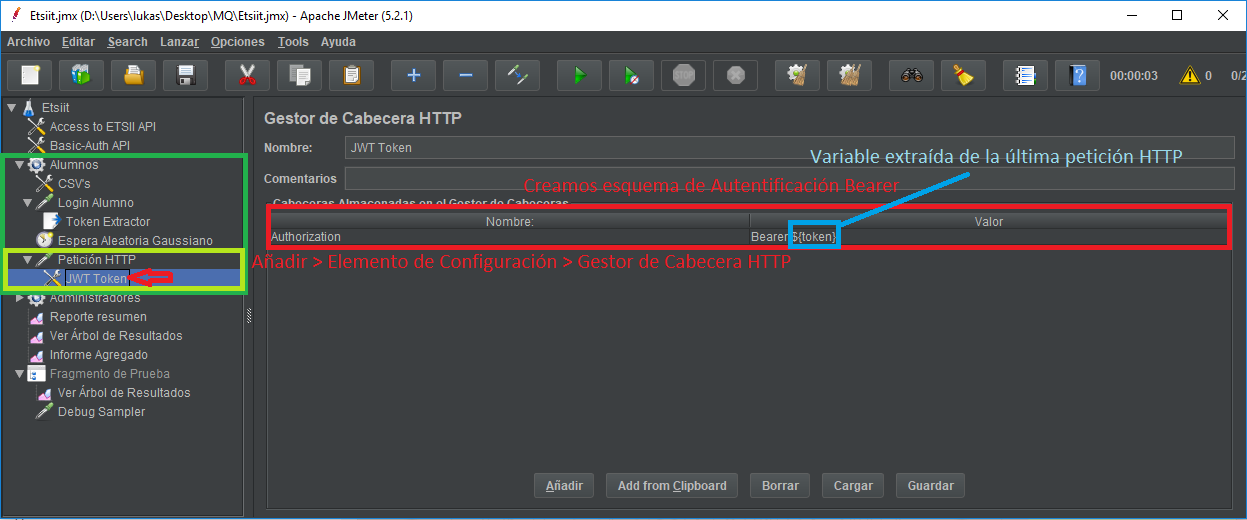
\includegraphics[width=1.0\textwidth]{images/step-9.png}
		\caption{Noveno paso, creación de variables del entorno}
	\end{figure}

	Para los administradores, a diferencia de los Alumnos de una única , van a realizar todas las peticiones que tiene el archivo \textbf{TCP Log} que vamos a utilizar sobre los Alumnos.
	

	\begin{figure}[h]
		\centering
		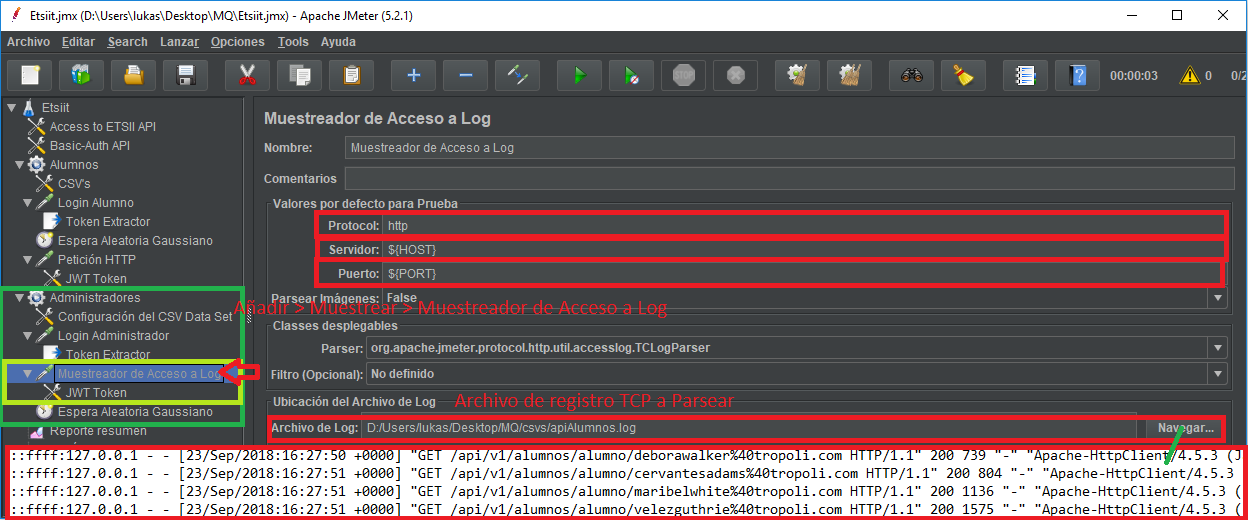
\includegraphics[width=1.0\textwidth]{images/step-10.png}
		\caption{Décimo paso, Muestreo TCP Log}
	\end{figure}
	\newpage
	Una vez acabado, podemos Añadir \textbf{Receptores} para visualizar los resultados.
	Podemos comprobar que no ha ocurrido ningún fallo viendo el árbol de peticiones, existen 5 códigos de resolución de una petición
	\begin{enumerate}
		\item {\color{info}\textbf{1**}} Respuestas informativas
		\item {\color{ok}\textbf{2**}} Respuestas satisfactorias
		\item {\color{redirection}\textbf{3**}} Redirecciones
		\item {\color{bad}\textbf{4**}} Errores de cliente
		\item {\color{bad}\textbf{5**}} Errores de servidor
	\end{enumerate}
	
	\begin{figure}[h]
		\centering
		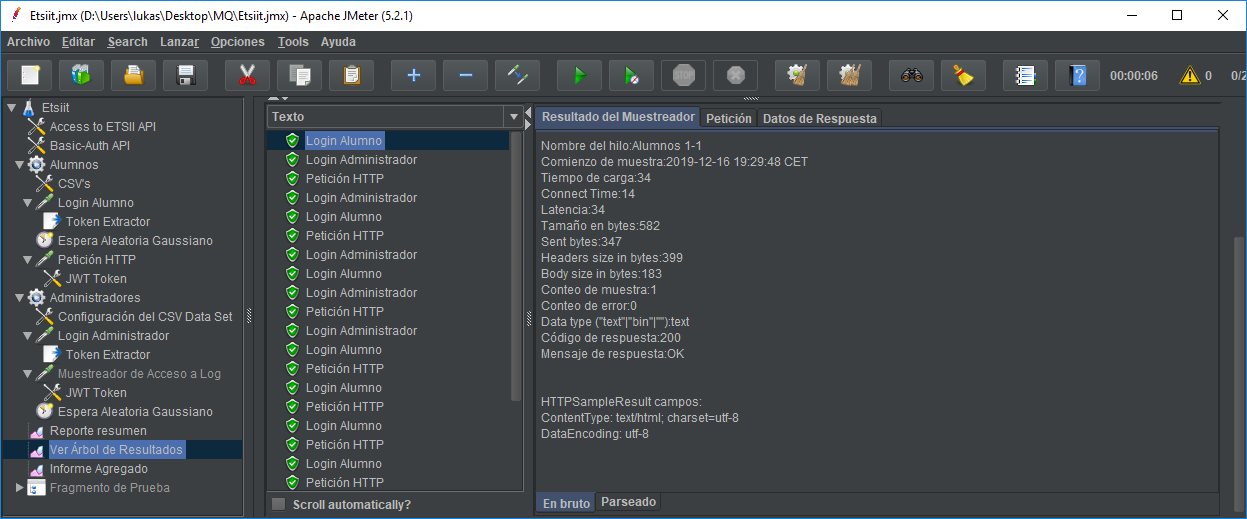
\includegraphics[width=0.9\textwidth]{images/tree-results.png}
		\caption{Árbol de peticiones}
	\end{figure}

	\begin{figure}[h]
		\centering
		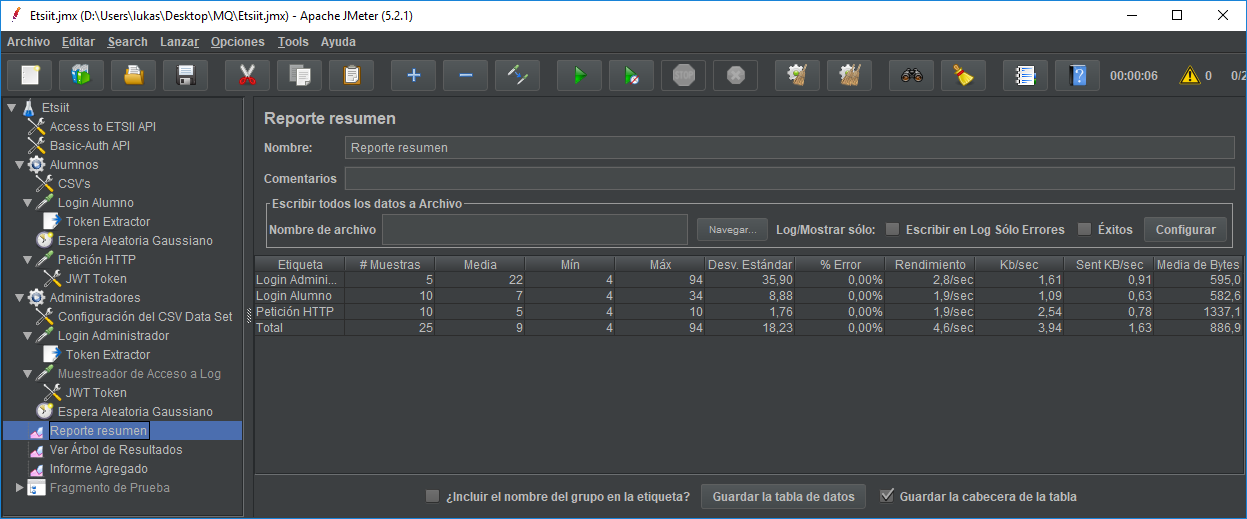
\includegraphics[width=0.9\textwidth]{images/summary-report.png}
		\caption{Resumen de las peticiones}
	\end{figure}
	
	\newpage
	\section{Referencias Bibliográficas}
	\begin{thebibliography}{9}
		
		\bibitem{Zabbix}
		Códigos de estado de respuesta HTTP
		\url{https://developer.mozilla.org/es/docs/Web/HTTP/Status}
		
	\end{thebibliography}
		
\end{document}